\section{Results}
\subsection{Pairwise Associations}
Table~\ref{tab:correlations} reports the strongest reproducible scalar-feature correlations. Rain absolute and rain accumulated each correlate with RSSI at $r=0.386$, SNR at $r=0.450$, and throughput at $r=0.312$. Pressure is negatively correlated with the same metrics ($r=-0.336$, $-0.433$, and $-0.267$). Latency has no individual association exceeding $|r|=0.084$. No $p$-values or confidence intervals were calculated in the repository.

\begin{table}[t]
\caption{Largest Reproduced Individual Pearson Correlations}
\label{tab:correlations}
\centering
\footnotesize
\begin{tabular}{llr}
\toprule
Target & Weather variable & $r$\\
\midrule
RSSI & Rain absolute/accumulated & $0.386$\\
     & Pressure & $-0.336$\\
     & Humidity & $-0.205$\\
SNR  & Rain absolute/accumulated & $0.450$\\
     & Pressure & $-0.433$\\
     & Wind speed & $-0.251$\\
Throughput & Rain absolute/accumulated & $0.312$\\
     & Pressure & $-0.267$\\
     & Humidity & $-0.228$\\
Latency & Wind direction & $-0.084$\\
     & Humidity & $0.053$\\
     & Rain absolute/accumulated & $-0.051$\\
\bottomrule
\end{tabular}
\end{table}


Stored trio tables report a rain-accumulated/pressure/rain-absolute average correlated with RSSI at $r=0.386$ ($R^2=0.149$) and SNR at $r=0.450$ ($R^2=0.203$). The best stored throughput trio---rain accumulated, rain absolute, and wind speed---has $r=0.314$ ($R^2=0.099$). The only retained latency trio has $r=-0.097$ ($R^2=0.009$). These averages mix units and include redundant rain fields, so they do not improve the physical interpretation over individual correlations.

\subsection{Predictive Models}
Table~\ref{tab:model-results} gives holdout results reproduced from the scripts. Polynomial regression is the strongest tested RSSI configuration ($R^2=0.190$, RMSE $=3.958$), while Lasso is strongest for SNR ($R^2=0.208$, RMSE $=3.077$) and throughput ($R^2=0.118$, RMSE $=16.115$). Every latency configuration is worse than the test-set mean baseline ($R^2<0$).

\begin{table*}[t]
\caption{Fixed-Holdout Regression Results Reproduced from Repository Scripts}
\label{tab:model-results}
\centering
\footnotesize
\begin{tabular}{lrr|rr|rr|rr}
\toprule
&\multicolumn{2}{c|}{RSSI}&\multicolumn{2}{c|}{SNR}&\multicolumn{2}{c|}{Throughput}&\multicolumn{2}{c}{Latency}\\
Model & $R^2$ & RMSE & $R^2$ & RMSE & $R^2$ & RMSE & $R^2$ & RMSE\\
\midrule
Linear & $0.173^{a}$ & $4.370$ & $0.201$ & $3.090$ & $0.107$ & $16.212$ & $-0.029$ & $0.063$\\
Polynomial (2) & $0.190$ & $3.958$ & $0.208$ & $3.077$ & $0.097$ & $16.303$ & $-0.050$ & $0.063$\\
Random forest & $0.004^{b}$ & $4.389$ & $0.061$ & $3.350$ & $-0.042$ & $17.509$ & $-0.039$ & $0.063$\\
Lasso & --- & --- & $0.208$ & $3.077$ & $0.118$ & $16.115$ & $-0.001$ & $0.062$\\
Ridge & --- & --- & $0.202$ & $3.087$ & $0.109$ & $16.191$ & $-0.028$ & $0.063$\\
KNN ($k=5$) & $0.046$ & $4.295$ & $0.057$ & $3.357$ & $-0.131$ & $18.248$ & $-0.065$ & $0.064$\\
\bottomrule
\end{tabular}

\raggedright\scriptsize $^{a}$RSSI linear regression uses a 10\% test split; other entries use 20\%. $^{b}$RSSI forest uses 200 trees; the other forests use 100. Dashes indicate that the repository has no corresponding RSSI configuration.
\end{table*}


For RSSI KNN, $k=9$ performs best among the four stored configurations, but remains weak ($R^2=0.099$). Figure~\ref{fig:knn} shows the contraction of predictions toward the center of the RSSI range. The repository also contains feature-coefficient/importances plots and predicted-versus-actual plots; only representative figures whose generating scripts are traceable are included here.

\begin{figure}[t]
\centering
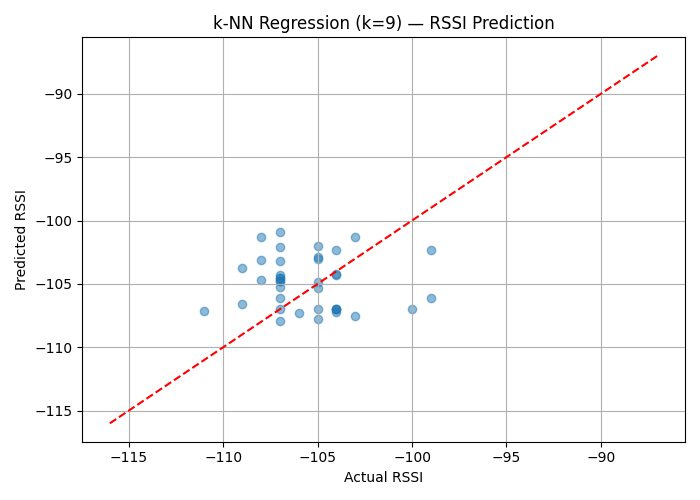
\includegraphics[width=\columnwidth]{knn_rssi_k9.png}
\caption{Actual versus predicted RSSI for KNN with $k=9$ on the fixed 20\% holdout. The dashed line denotes perfect prediction.}
\label{fig:knn}
\end{figure}

\begin{figure}[t]
\centering
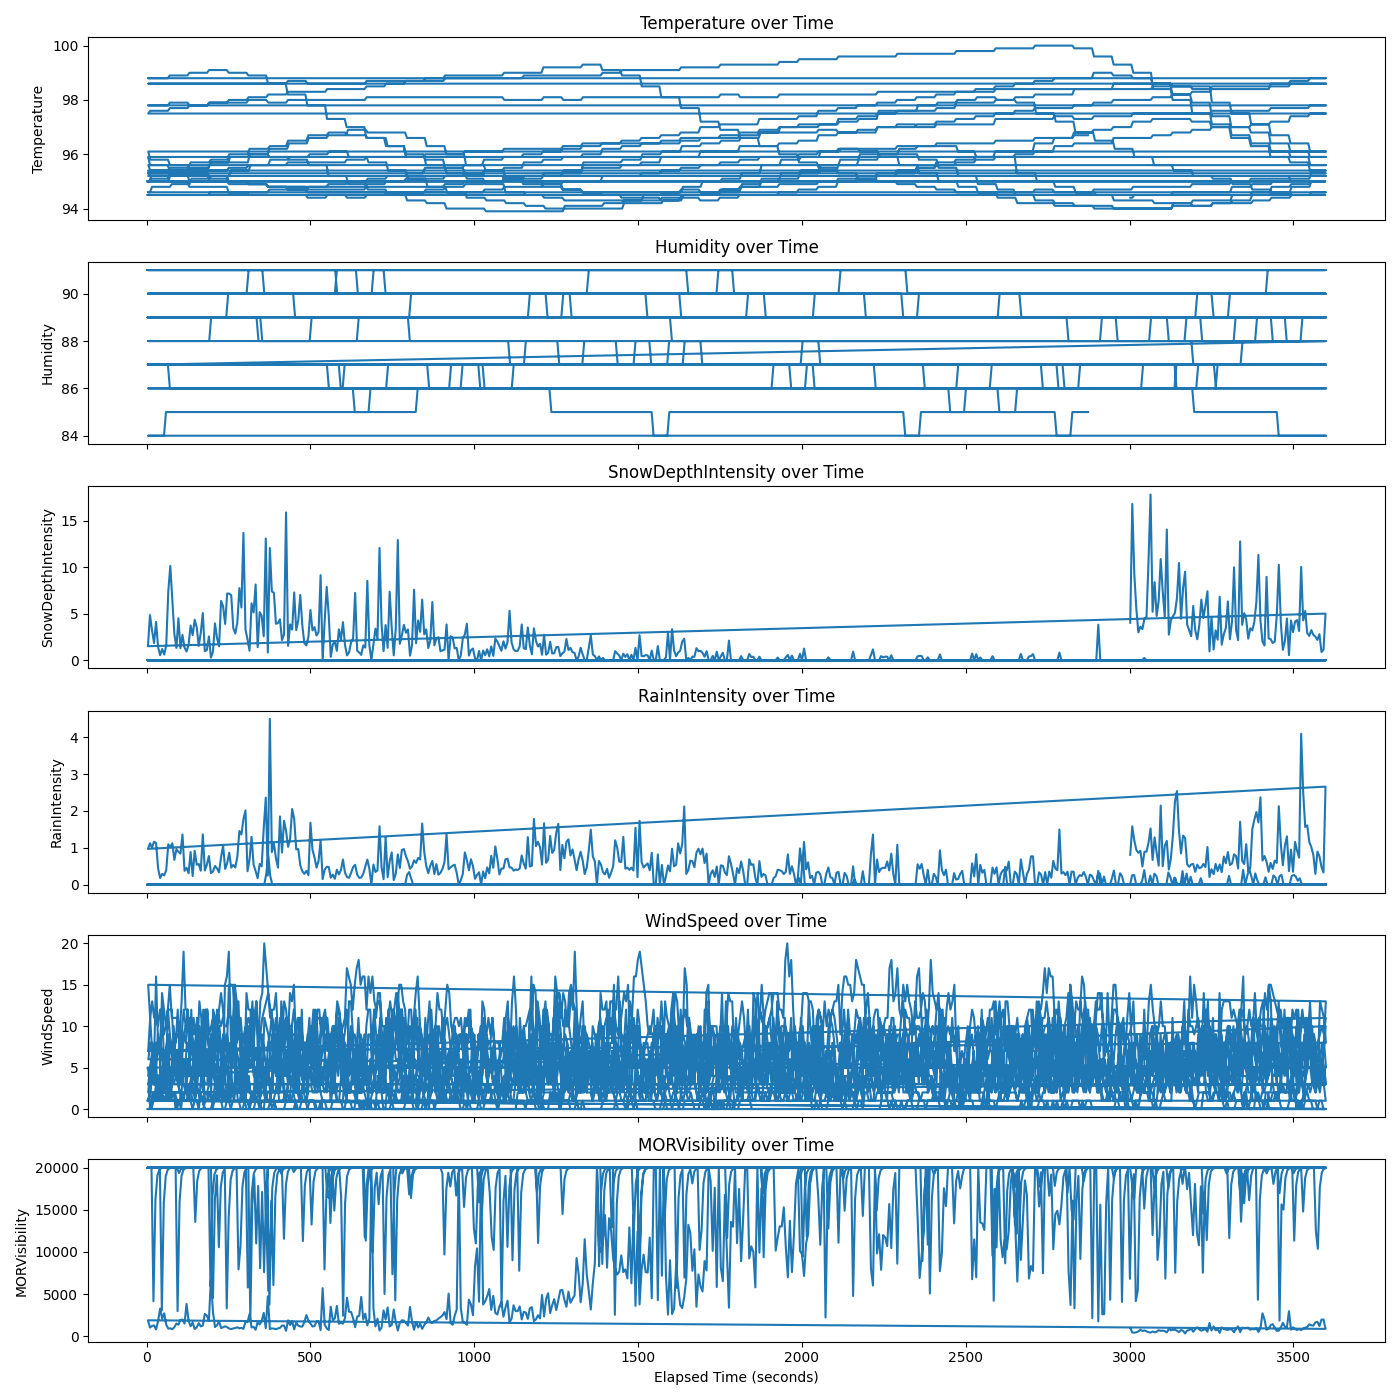
\includegraphics[width=\columnwidth]{weather_metrics_plot.png}
\caption{Repository-generated weather time series for the December 17--18 snow-session file. The source script plots temperature, humidity, snow-depth intensity, rain intensity, wind speed, and MOR visibility. Units are undocumented.}
\label{fig:weather}
\end{figure}
